\chapter{Results and Discussion}
This chapter explains the validation infrastructure built around the implemented design and shows the functional correctness of several corner cases. Afterwards it reports on the results obtained after synthesis and implementation and finally discusses these results.





\section{Validation Framework}
\label{sec:verif}
The validation framework consists of three modules to automatically test if the implemented design is functionally correct, shown in \autoref{fig:8-validation}. This simplifies validation of adjustments to the design, but also different configurations of the design.\\
The diagram follows the conventions mentioned in Section \ref{sec:legend} but adds a yellow rounded rectangle for validation modules. The function of each of the modules will be briefly discussed.

\begin{figure}[H]
  \centering
  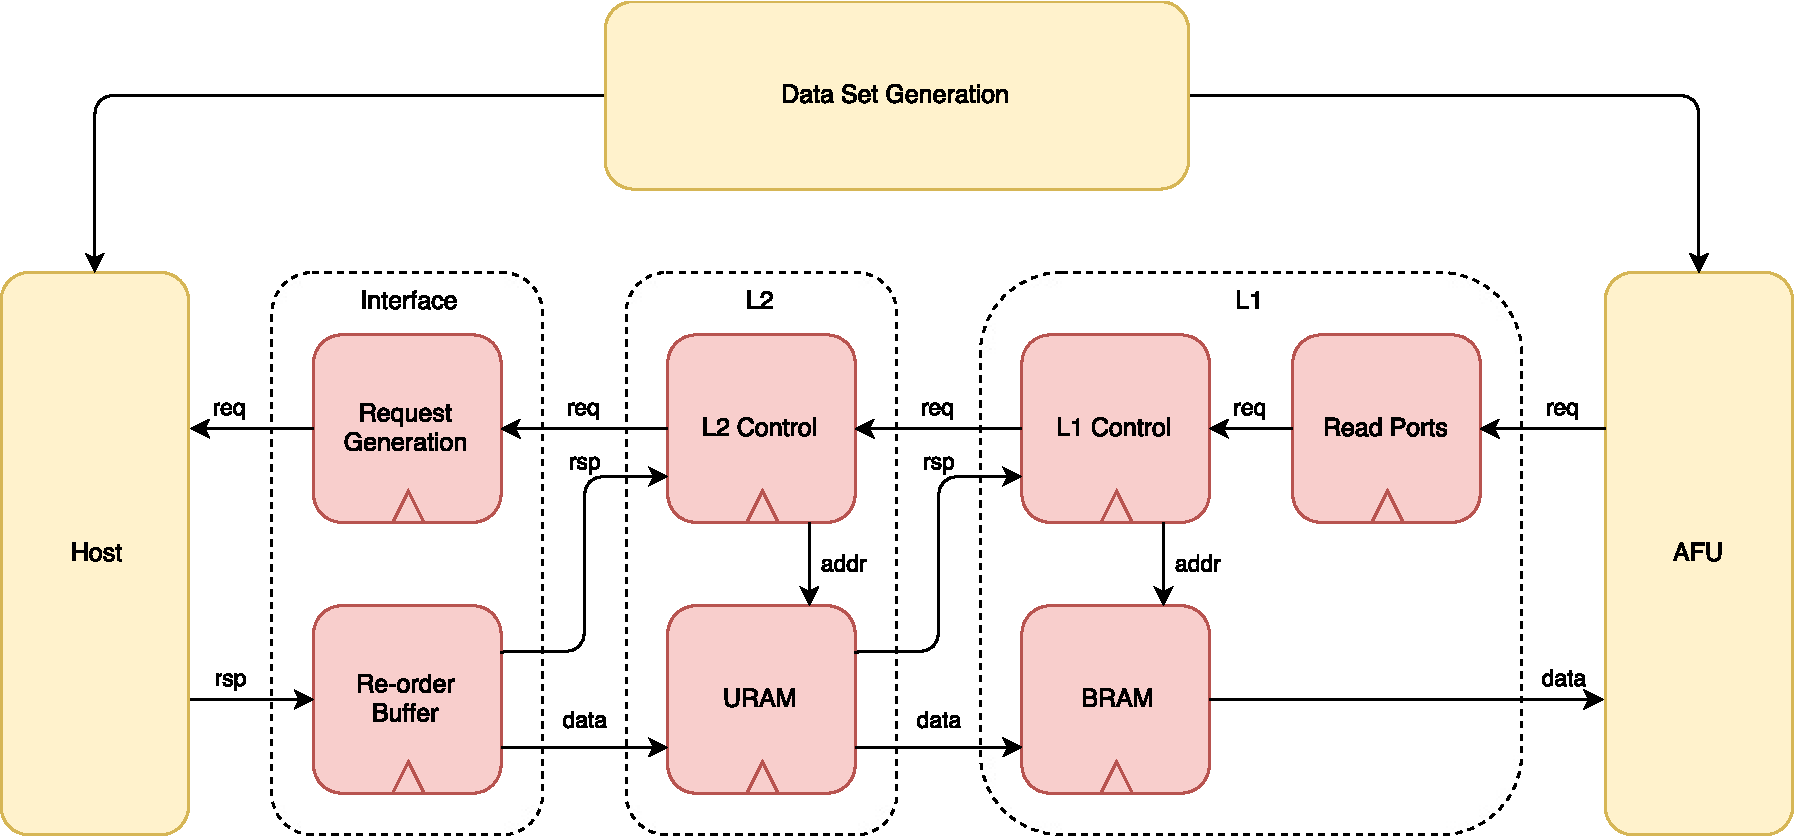
\includegraphics[width=0.95\textwidth]{8-verification.pdf}
  \caption{Diagram of the validation framework.}
  \label{fig:8-validation}
\end{figure}



\subsection{Data Set Generation Module}
The function of this module is to generate a data set that acts as the stream data found in host memory. Cache lines have to be written in two half cycles and \SI{16}{\byte} data elements are distributed between two physical addresses. Therefore, the data generation module initially generates a two-dimensional array with a number of entries equal to twice the number of data elements required for all streams combined, with a data width of half a data element or \SI{8}{\byte}. This array is then shuffled into an array usable for the Host module and for the AFU module.\\
The Host module will write a new cache line to the URAM module in two half cycles. Therefore, the initially generated data has to be shuffled to obtain a two-dimensional array with the number of entries equal to twice the number of cache lines required for all streams combined, with a data width of half a cache line or \SI{64}{\byte}. Each entry is a concatenation of eight half-sized data elements, either the even or odd indexed half data element from the original data set.\\
The AFU module also needs a shuffled version of the initial data set, but is different compared to the Host module. The reason is that the AFU module has to compare one or multiple data elements of \SI{16}{\byte}, depending on the configuration received from the BRAM module or modules. The new two-dimensional array has the number of entries equal to the number of cache lines required for all streams combined, with a data width of a cache line or \SI{128}{\byte}.



\subsection{Host Module}
The Host module consists of a register cell with a latency of one clock cycle that loops back the request made by the \textit{Request Generation} module to the \textit{Re-order Buffer} module. The number of cycles can be adjusted, depending on the host architecture.\\
When a valid request is received and the Host module is ready to accept, a task is initiated to write the next cache line for the requested stream into the URAM module. The Host module has a counter per stream to index the provided data set by the Data Set Generation module and updates the counter accordingly.

%\todo{- Note that in the current implementation, the response from the Host to the L2 Control might not be synchronised with the write operation of the URAMs. This should be checked.\\}



\subsection{AFU Module}
The AFU module generates read requests for the \textit{Read Ports} module by initiating a task that has the read port and stream identifier as arguments. Each read request interface consists of a ready-valid signal pair and a stream identifier.\\
The module also validates data received from the BRAM array. Since each individual read port operates in-order, but read ports among each other do not, some logic keeps track of which read ports received valid data this cycle and updates counters per stream accordingly. These counters are used to index the shuffled data set provided by the Data Set Generation module.\\
Since read requests can be discarded for various reasons, the AFU module also keeps global counters of the number of read requests made per stream and the number of valid data elements received. When the test bench terminates, a summary of these counters per stream is printed. It can then be assessed if reads have been discarded as intended, for example when reading after a stream has ended, or if a discard has occurred due to a bug.



\subsection{Setup and Operation of a Stream}
Before using the multi-stream buffer, the circuit has to be reset first. After this has occurred, the Host and AFU modules indicate that they are ready to receive requests and data. In one cycle, only a single stream can be functionally reset. This is done by sending a request to the functional reset interface consisting of a ready-valid signal pair, a stream identifier, and a begin and end EA. The EA should point to a \SI{128}{\byte} aligned (required due to the direct-mapping of EAs to memory addresses). If the request is accepted, the L1 and L2 Control modules will start to request cache lines from the Host module by using the begin EA and fill their associate memory arrays. At any point after the functional reset request has been accepted, the AFU is allowed to make a read request for that particular stream. Depending on how many cache lines are valid in the BRAM arrays, the read request will be serviced right away or has to wait until there is enough valid data to continue.\\
The begin EA is recalculated according to requests made to the Host module. When the begin EA surpasses the end EA, the stream has ended. This means that both the BRAM and URAM arrays still have valid data, so until there is no more valid data available, read requests for that stream will be accepted. The output functional reset interface will indicate when the stream has entirely ended. At this point, read requests made will be discarded and the AFU should use the read port to request unfinished streams, or functionally restart the stream again.





\section{Functional validation}
With the validation framework in place, changing the implementation and its functional validation is as easy as pressing a button. This allows to quickly functionally verify different configurations and corner case access patterns. This section visualizes various access patterns, proves the L1 buffer size analysis, and validates corner cases.

\subsection{Multi-Read Port Access Patterns}
To not overwhelm the reader, the configuration is slightly tuned down to 32 streams, four read ports, and two write channels. Section \ref{sec:boundary} showed four distinct access patterns possible for a configuration with eight read ports and eight data elements per cache line. The configuration used has four read ports and the same number of data elements per cache line, but this still allows us to show the correct operation of these access patterns.\\
\autoref{fig:8-verif-1} shows the waveform of the four access patterns. The signal list contains both clock signals, the AFU read request interface showing the ready and valid signals and the stream identifier associated with each read port. Similarly the data response from the BRAM arrays is shown, accompanied by the ready and valid signals, and the stream identifiers. Also the cache line offset and cache line number are shown for stream five, six and seven. Note that the time dimension is not to scale.

\subsubsection{All Reads from a Single Stream}
The leftmost marker indicates the start of an access pattern where all read ports request the same stream. The data response with the associated stream identifiers appears five cycles later. Currently the first cache line is read and the starting offset is three. This is due to the fact that this stream was read at an earlier stage to position the stream pointer at the desired offset within the cache line to demonstrate other access patterns. There is a cycle latency between the AFU read request and the offset update, since the AFU read request first flows through an input register.

\subsubsection{All Reads from Different Streams}
The second marker indicates the start of an access pattern where all read ports request different streams. The response contains data from the expected streams. Similarly as in the previous access pattern, the streams have been read at an earlier stage. Therefore the starting offset is six and since one read request is made per stream, the new offset is seven.

\subsubsection{Crossing a Cache Line Boundary}
The third marker indicates the start of an access pattern where a cache line boundary is crossed. Currently, the offset is seven. Therefore when four requests for this stream are made, the first request reads at offset eight and the other three requests read the first three elements from cache line one. This can be seen from the cache line offset and cache line identifier signals.

\subsubsection{Crossing Multiple Cache Line Boundaries}
The last marker indicates the start of an access pattern where two cache line boundaries are crossed. Similarly to previous patterns, some requests are made at an earlier stage. Therefore, the current offset is at seven for both streams six and seven. After making two read requests per stream, both offset seven from cache line zero and offset zero from cache line one are read.

\begin{figure}[H]
  \centering
  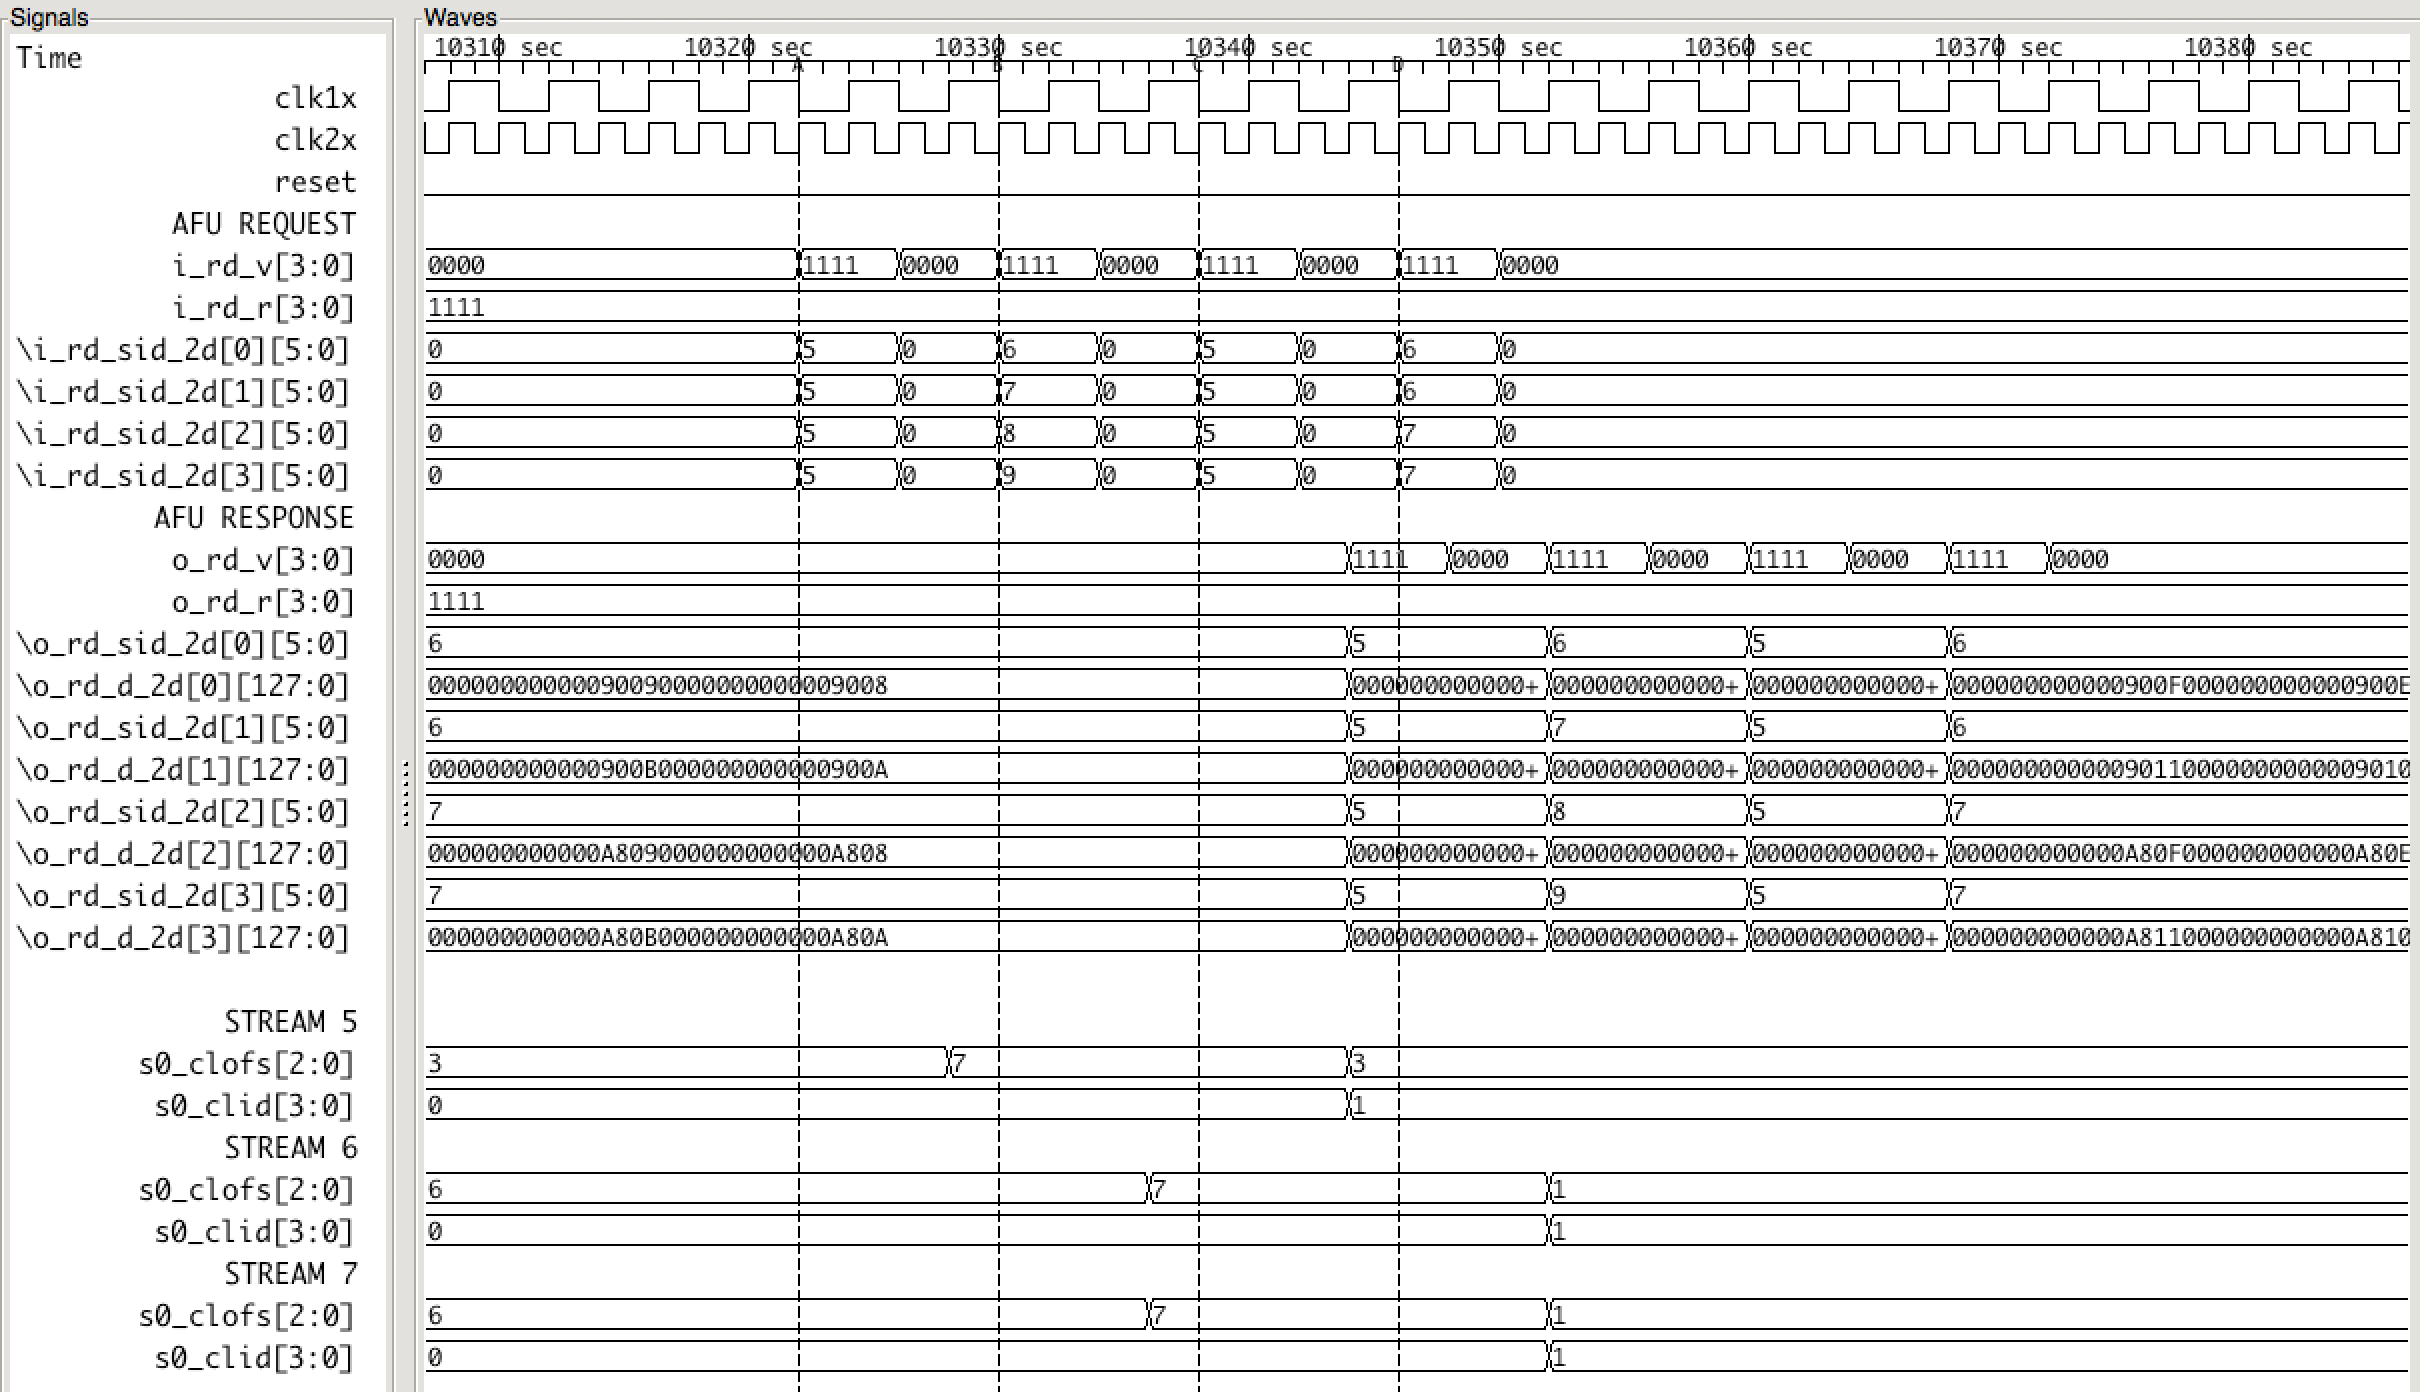
\includegraphics[width=0.95\textwidth]{8-verif-1.png}
  \caption{Waveform showing four distinct AFU access patterns.}
  \label{fig:8-verif-1}
\end{figure}



\subsection{L1 Buffer Depth validation}
Section \ref{sec:buffer} analyzed the required L1 buffer depth for any configuration. When using the desired configuration parameters in \autoref{eq:s}, latency \textit{L} is the only unknown parameter. Chapter 7 discussed the implementation in detail and therefore the latency is known. Latency \textit{L} is defined as the latency between the \textit{L2 Control} module accepting an L2 request from L1, to committing the new cache line in the BRAM slice. The L2 stream pointer has a latency of one cycle, followed by one cycle latency of the Round-Robin multiplexer, followed in turn by three cycles in the URAM slice, and finally one cycle to commit the new cache line. Therefore latency \textit{L} equals six clock cycles.\\
\autoref{tab:est} showed that a configuration with four write channels should have a buffer size of $L + 16$ to accommodate for the worst case access pattern. The closest power of two is sixteen and therefore this many entries was chosen. However, taking latency \textit{L} into account, the buffer size of each L1 stream should be 22 cache lines deep. This means that under the worst case access pattern and the assumption that no back-pressure will occur during run-time, six cycles of AFU read requests cannot be serviced. Depending on the access pattern of the AFU, this may or may not be a problem.

\subsubsection{Functional Simulation}
To illustrate this, a functional simulation was done and the results are shown in \autoref{fig:8-verif-2}. The signal window shows AFU read requests, the number of L1 valid and requested cache lines for stream fifteen, and the output of the Round-Robin multiplexer that arbitrates between sixteen streams to schedule read access.\\
The leftmost marker shows the moment L2 requests are triggered using the burst access pattern as described in Section \ref{sec:buffer-depth}. The next marker shows the start of the distributed access pattern. During the second cycle of the burst access pattern, the last element of each cache line is read. This is reflected by the number of valid cache lines signal \texttt{s0\_ncl} in stream fifteen, since it is reduced from sixteen to fifteen. During the following cycles, a full cache line is read from stream fifteen and the valid counter decreases by one every cycle.

\begin{figure}[H]
  \centering
  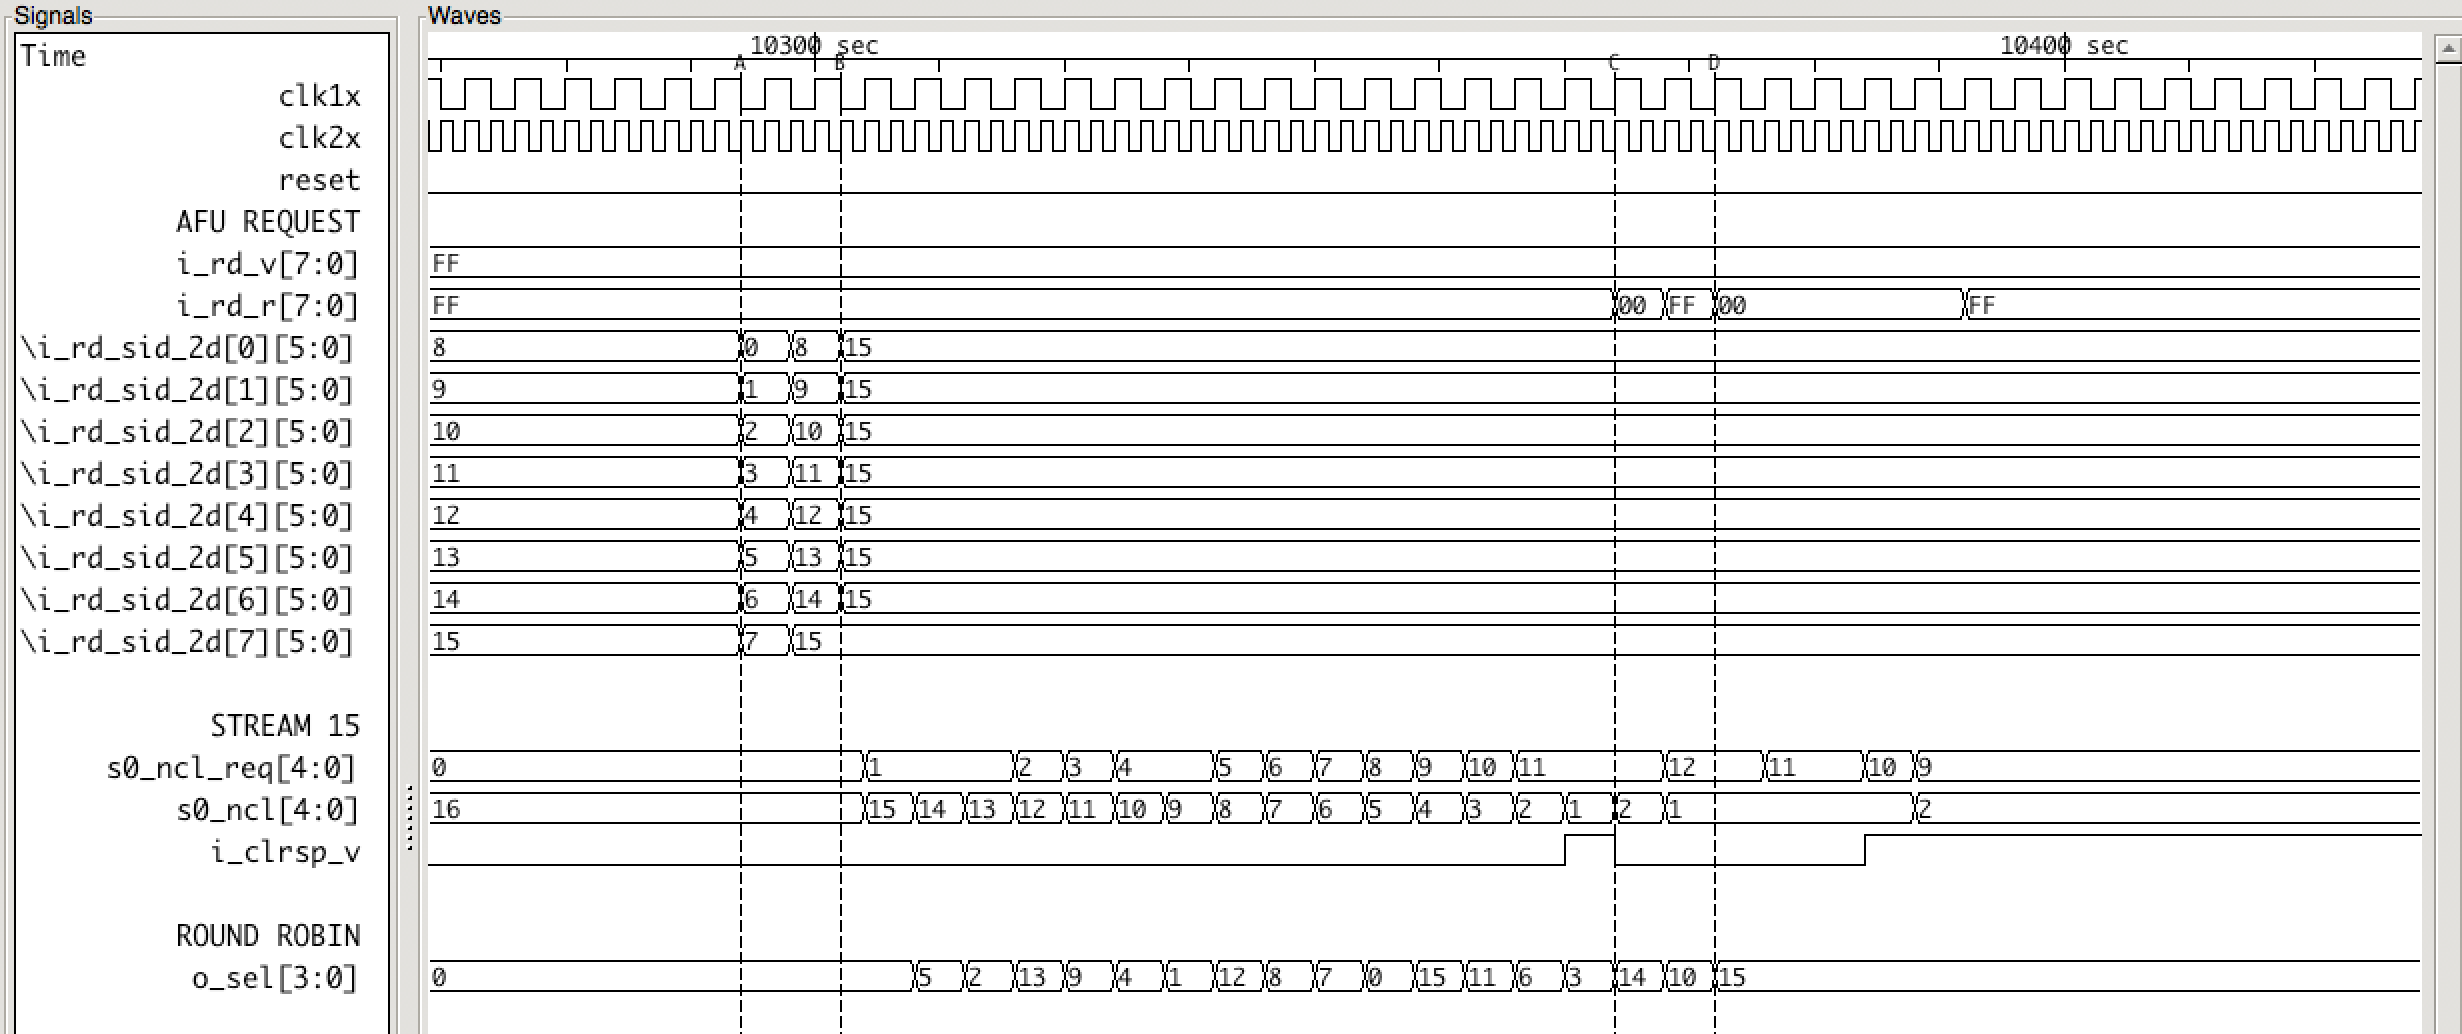
\includegraphics[width=0.95\textwidth]{8-verif-2.png}
  \caption{Waveform showing the worst case access pattern and the impact of the buffer size.}
  \label{fig:8-verif-2}
\end{figure}

\subsubsection{Discrepancy Between Analysis and Functional Simulation}
The model used during the analysis assumed that L2 requests would be serviced in ascending order. Due to the nature of the Round-Robin multiplexer, the request for stream fifteen is scheduled earlier as shown in the waveform by signal \texttt{o\_sel}, the output select signal of the Round-Robin multiplexer. As a consequence, a valid response \texttt{i\_clrsp\_v} for stream fifteen is received earlier than expected during analysis.\\
As expected, no AFU read requests are serviced for several cycles since the buffer is too small to handle this configuration. The third marker shows the first occurrence of this, when all read ports apply back-pressure to the AFU. Even though there is still one valid cache line present, read requests are only serviced when two or more valid cache lines are present to service access patterns that cross a cache line boundary, as mentioned before. Since the Round-Robin multiplexer scheduled stream fifteen earlier than expected in the analysis model, the valid counter is briefly incremented to two valid cache lines, which then removes the back-pressure. The forth marker indicates the second time back-pressure is applied for the same reason. In total, back-pressure is applied for six cycles. This is in accordance with the expectation to facilitate this access pattern without any loss in performance, the buffer should have had 22 entries. Instead the buffer contains sixteen entries and consequently no AFU read requests are accepted for six cycles.



\subsection{Discarding Read Requests to Prevent Deadlocks}
Section \ref{sec:deadlocks} discussed three conditions for which incoming read requests from the AFU should be discarded in order to prevent deadlocks. This paragraph validates this behavior by simulating the conditions.

\subsubsection{Servicing Read Requests before Functional Reset}
Section \ref{sec:deadlocks} mentioned that servicing read requests before a functional reset, or after a stream has terminated, results in a discarded request. No valid data is present and therefore no read requests are allowed.\\
\autoref{fig:8-verif-3} shows the AFU request interface. The leftmost marker indicates a read request on read port one and the second marker indicates the same signal after the input register. Since the \texttt{invalidate\_rd} signal is high, meaning that the request stream has not yet been reset (or has ended), the read request is discarded. Therefore the next downstream signal \texttt{s1\_rd\_v} is de-asserted.\\
Since this implementation also discards a read request when it is issued after the stream has terminated, no waveform is shown for this corner case.

\begin{figure}[H]
  \centering
  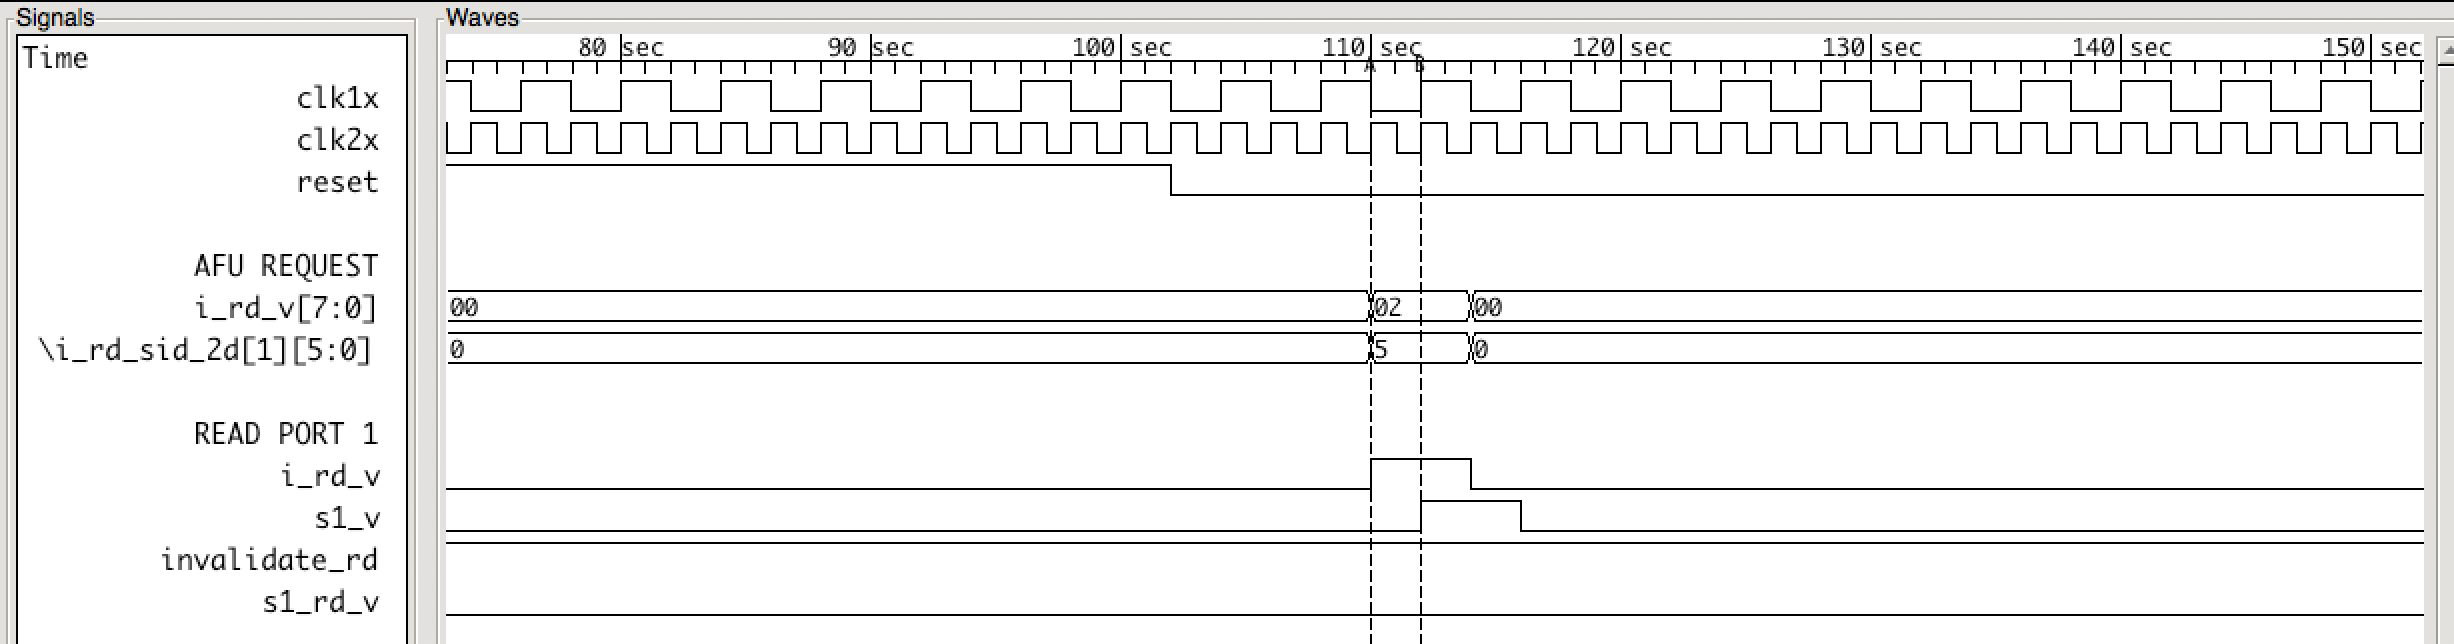
\includegraphics[width=0.95\textwidth]{8-verif-3.png}
  \caption{Waveform shows read request discard when issued before a functional reset.}
  \label{fig:8-verif-3}
\end{figure}

\subsubsection{Termination of a Stream Mid-Cycle}
Another discard condition is when multiple requests are made during the same cycle, but within that cycle the last element from the stream is read. Therefore, one or multiple read requests have to be discarded since no more valid data is present.\\
\autoref{fig:8-verif-4} shows the AFU request and response interface, followed by internal signals of stream five, and read port zero and one signals. The leftmost marker indicates an AFU read request on two ports, both for stream five. Stream five is currently at offset seven, with one valid cache line left. The second marker indicates the same signal after the input register (\texttt{s1\_rd\_v}). The out-of-bounds signal tests if the stream has ended and a request is made. If this is the case, as is in this example, the signal is asserted. This de-asserts the input valid signal \texttt{s1\_rd\_v\_test} to the combine cell in the read port logic and therefore the read request is discarded.\\
Read port one, however, does not discard the read request because it will service the element at offset seven. Therefore the AFU response interface shows one valid output at the fourth marker. This valid signal belongs to read port zero, as expected.

\begin{figure}[H]
  \centering
  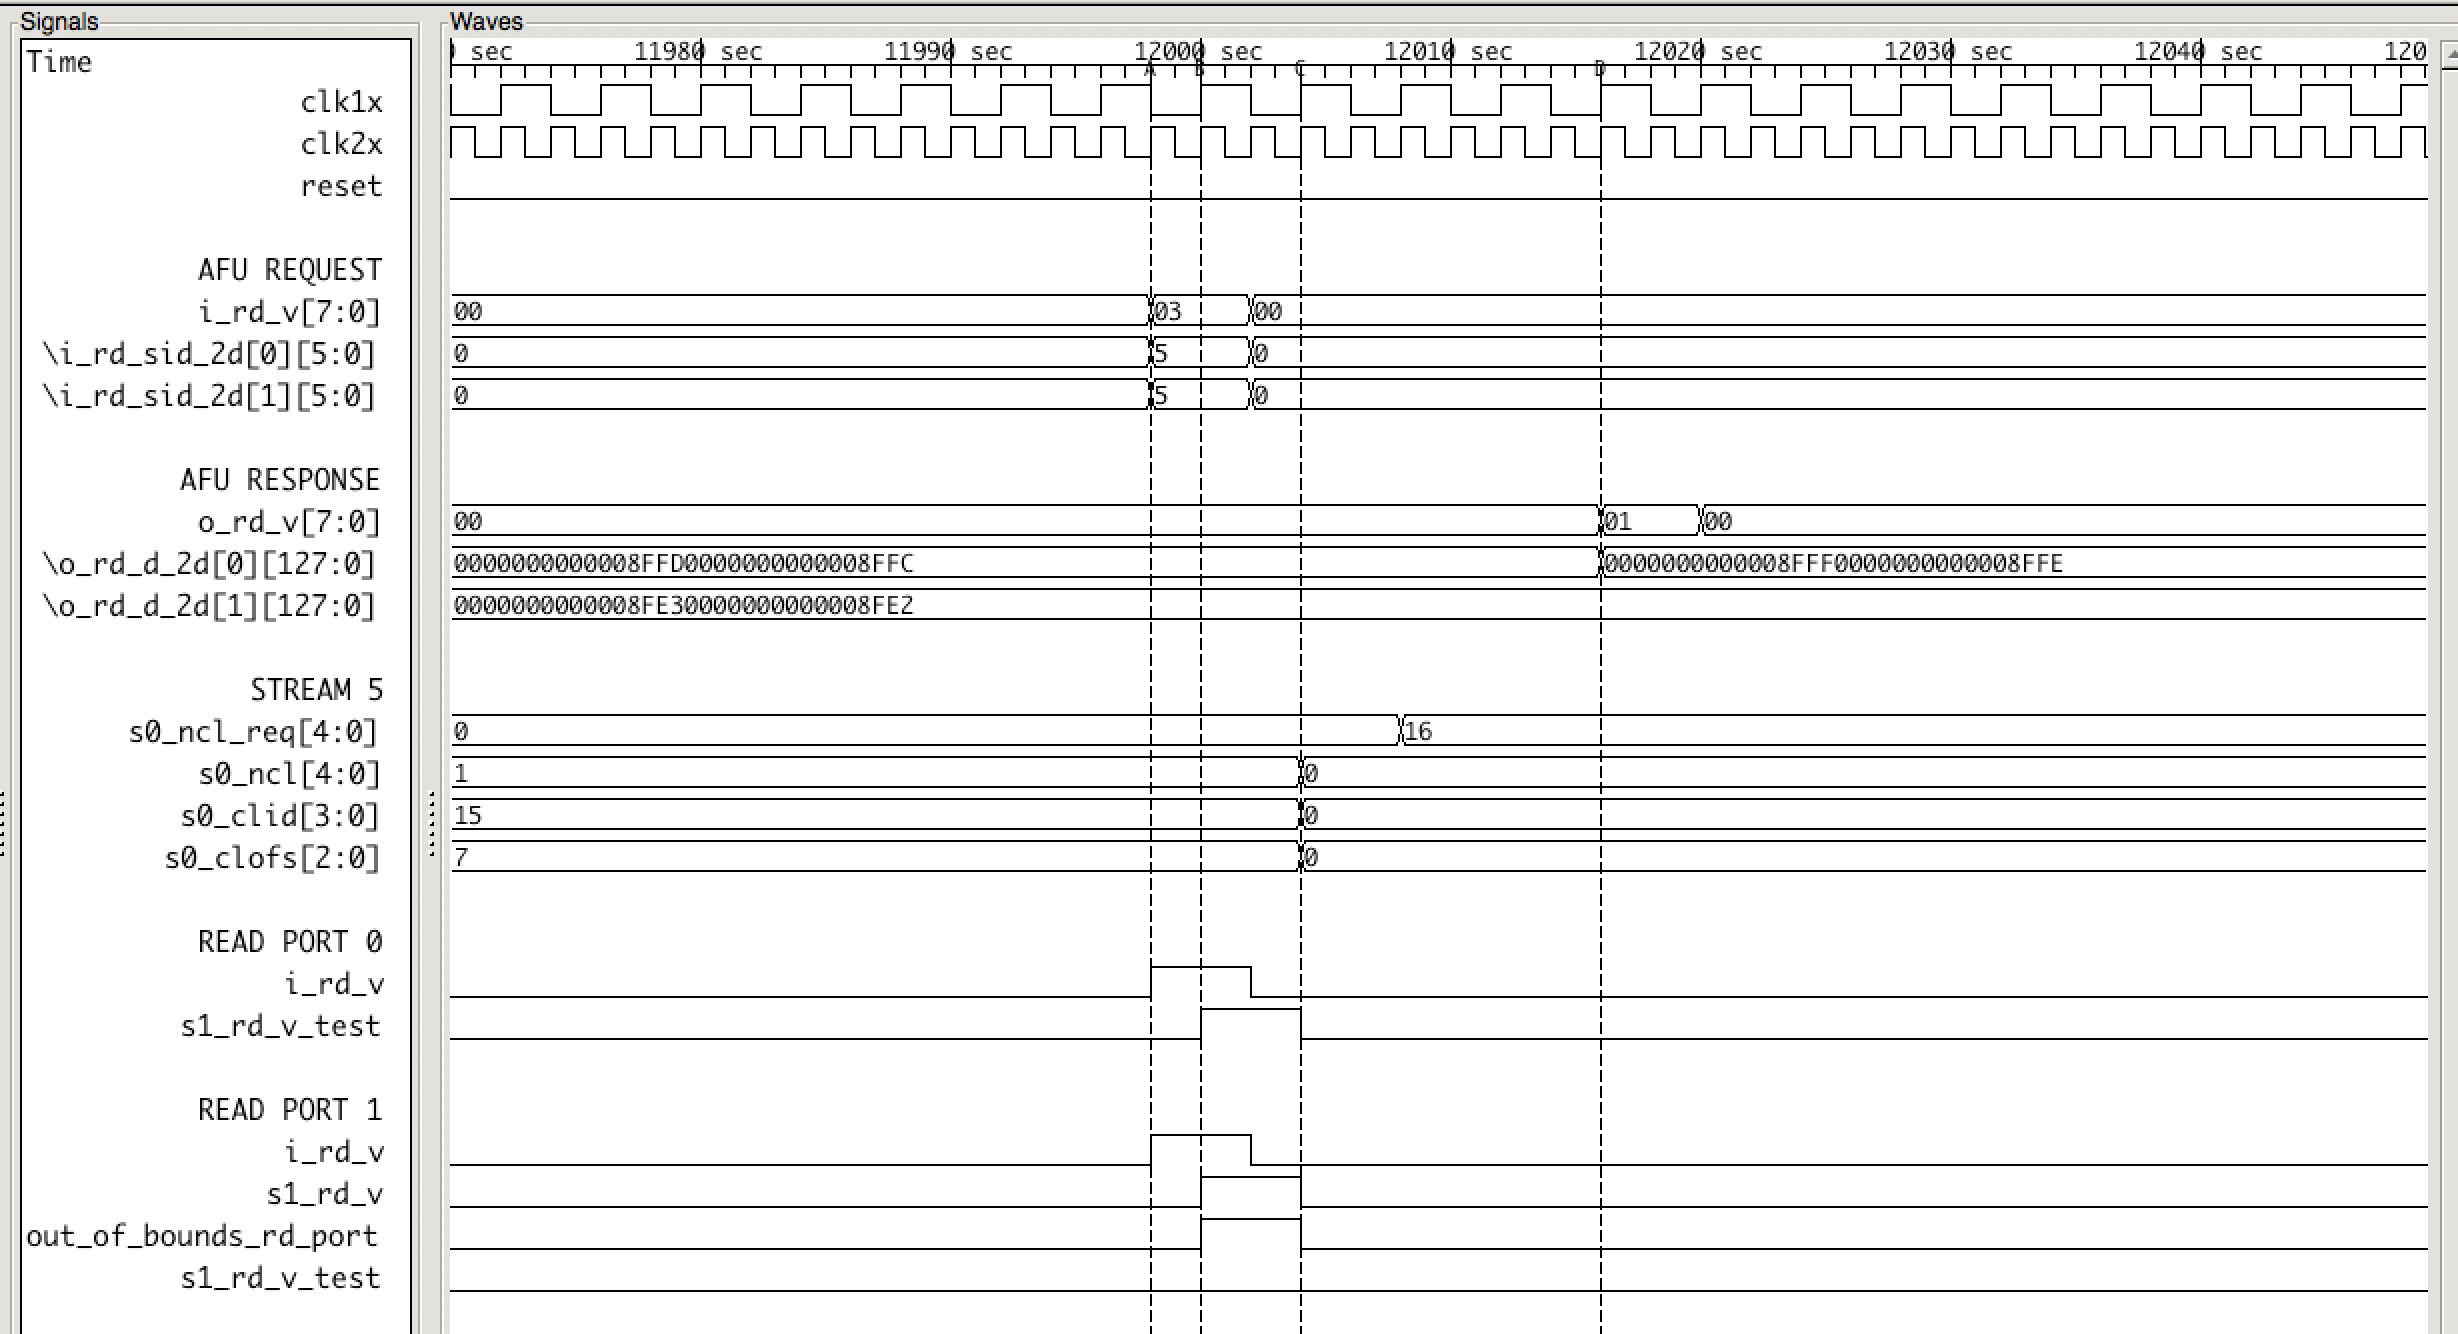
\includegraphics[width=0.95\textwidth]{8-verif-4.png}
  \caption{Waveform shows read request discard when stream terminates mid-cycle.}
  \label{fig:8-verif-4}
\end{figure}





\section{Synthesis and Implementation Results}
Besides functional validation, the design has to be synthesized and implemented as well to verify the operating frequency and resource utilization. First the setup of the Vivado 2017.1 toolchain is explained and afterwards the obtained results for various configurations are presented.



\subsection{Vivado Toolchain Setup}
Since the multi-stream buffer is a sub-module in a larger design, obtaining implementation results such as resource utilization and timing is complex and with uncertainty. Typically an FPGA design is connected to the physical pins on the chip's package. Since this is not the case here, the tool has to be instructed neither to route wires to these pins, nor take the wires into account during timing analysis. Vivado provides a special mode for such an isolated approach called \texttt{out\_of\_context}. This mode is used to obtain the results presented below.\\
Typically, input and output signal constraints are provided, but this increases implementation time dramatically. It has happened that the implementation phase increased from 15 min to 5 hours for a small configuration of the design. Since all inputs go directly to registers and all outputs come directly off registers, no constraints are applied. Since an input signal constraint would only check the path from the pin to the directly connected register, such a test is basically meaningless. There is no logic and therefore it cannot be the critical path. The critical path is between the input and output registers and it is thus sufficient to specify clocks only.\\
All clocks are related by default. The two clocks used for the final design will come from the clock source. To make sure the tools include clock skew, an additional \textit{hierarchical design} constraint related to the clock source is added. With this constraint the tools know which source is driving the clock. In the future, both clocks are expected to be driven by buffers, therefore a different buffer is chosen for each clock constraint.\\
One of the downsides of the \texttt{out\_of\_context} mode is that it will typically only indicate a best case scenario. When a sub-module is integrated in the final design, particularly when the design consumes a significant part of the available resources, the reported performance of the sub-module will be at best the results obtained in the \text{out\_of\_context} mode \cite{xilinx-forum}.



\subsection{Synthesis Results}
Using the described Vivado toolchain setup, various configurations of the multi-stream buffer have been synthesized and implemented. Both the synthesis and implementation target the KU15P using the Vivado 2017. Since several versions are available within Vivado, the lowest-end part regarding temperature and speed grade is chosen to allow for variations (\texttt{xcku15p-ffve1760-1-e}).\\
In order to help FPGA designers with a specific workflow, Vivado provides various synthesis strategies. Strategies range from fast results to performance optimized. The latter is chosen for this project, in order to let the tool help as much as possible to obtain the target frequencies. For that reason, the \texttt{Flow\_PerfOptimized\_high} is chosen and turns off resource sharing, and decreases the maximum fan-out for example.\\
The timing constraints are set to \SI{200}{\mega\hertz} and \SI{400}{\mega\hertz}, respectively. When the tool finds a solution that fits the timing constraints, it will no longer continue to search for a possibly better alternative. Additionally, typically the timing constraints are higher than your actual target frequency because in an FPGA the wire routing delay will be dominant. To accommodate for both, usually a design is over-constrained. To find an optimum between the level of confidence that the design will work, and the run-time of the tool, the design is not over-constrained.\\
The synthesis results of various configurations are shown in \autoref{tab:synth1} and \autoref{tab:synth2}. The same parameter naming scheme is used as in \autoref{eq:s}. Table entry \textit{N} indicates the total number of streams, \textit{C} indicates the number of channels, \textit{P} indicates the number of read ports, \textit{F} indicates the \texttt{clk1x} constraint, \textit{WNS} shows the worst negative slack, \textit{WHS} shows the worst hold slack, and \textit{WPWS} shows the worst pulse width slack.\\
To reduce run-time of the tool, the number of L2 cache lines per stream is decreased from 256 to 128. Getting data out of the memory columns and the fan-out from the URAM to the BRAM slices that increases with the number of read ports are the most difficult parts of the design to place and route. These complexities are still present, even with this reduction in cache lines.

%\todo{- Overconstrain configurations.}

\begin{table}[H]
  \centering
  \caption{Synthesis timing and power consumption results for various configurations.}
  \label{tab:synth1}
  \begin{tabular}{ c | c | c || c || c | c | c || c }
    \textbf{N} & \textbf{C} & \textbf{P} & \textbf{F [MHz]} & \textbf{WNS [ns]} & \textbf{WHS [ns]} & \textbf{WPWS [ns]} & \textbf{Power [W]} \\ \hline \hline
    %32 & 2 & 2 & xxx & x.xxx & x.xxx & x.xxx & x.xx \\
    32 & 2 & 4 & 200 & 0.761 & 0.049 & 0.412 & 2.784 \\
    32 & 2 & 8 & 200 & 0.761 & 0.049 & 0.412 & 4.085 \\
    64 & 4 & 4 & 200 & 0.761 & 0.049 & 0.412 & 4.707 \\
    64 & 4 & 8 & 200 & 0.761 & 0.049 & 0.412 & 7.226 \\
  \end{tabular}
\end{table}

\begin{table}[H]
  \centering
  \caption{Synthesis resource utilization for various configurations.}
  \label{tab:synth2}
  \begin{tabular}{ c | c | c || c || c | c | c | c }
%    \textbf{CLB LUTs} & \textbf{CLB Registers} & \textbf{LUT as Memory} & \textbf{BRAM} & \textbf{URAM} \\ \hline \hline
%    11097 (2.12\%) & 12245 (1.17\%) & 0 (0.00\%) & 72 (7.32\%) & 16 (12.50\%) \\
%    14195 (2.72\%) & 15185 (1.45\%) & 0 (0.00\%) & 144 (14.63\%) & 16 (12.50\%) \\

    \textbf{N} & \textbf{C} & \textbf{P} & \textbf{F [MHz]} & \textbf{CLB LUTs} & \textbf{CLB Registers} & \textbf{BRAM} & \textbf{URAM} \\ \hline \hline
    32 & 2 & 4 & 200 & 11274 (2.16\%) & 13329 (1.27\%) & 72 (7.32\%) & 16 (12.50\%) \\
    32 & 2 & 8 & 200 & 14195 (2.72\%) & 15185 (1.45\%) & 144 (14.63\%) & 16 (12.50\%) \\
    64 & 4 & 4 & 200 & 23286 (4.45\%) & 25205 (2.41\%) & 136 (13.82\%) & 32 (25.00\%) \\
    64 & 4 & 8 & 200 & 28667 (5.48\%) & 28248 (2.70\%) & 272 (27.64\%) & 32 (25.00\%) \\
  \end{tabular}
\end{table}

For each configuration, the synthesis tool reports that the timing constraints are met and the resource utilization is in line with the expectations. The number of BRAMs is slightly higher than expected. Since each BRAM slice requires a credit sink cell, a First-In-First-Out (FIFO) cell is used which uses a memory. Since the data width is equal to the data element width, two BRAMs are required per FIFO.\\
The longest path for each configuration is the internal path between a URAM array and an internal pipeline stage. However, the slack will dramatically decrease during implementation.



\subsection{Implementation Results}
After several initial implementation runs, it became apparent that small tweaks had to be made to the original design. The timing constraints where not met, even after several hours. While the synthesis results where promising with respect to meeting the timing constraints, the influence of the inherent location of memory primitives in columns became quickly clear. \autoref{tab:synth3} and \autoref{tab:synth4} summarize the obtained results for the same configurations as shown in the previous section.

\begin{table}[H]
  \centering
  \caption{Implementation timing and power consumption results for various configurations.}
  \label{tab:synth3}
  \begin{tabular}{ c | c | c || c || c | c | c || c }
    \textbf{N} & \textbf{C} & \textbf{P} & \textbf{F [MHz]} & \textbf{WNS [ns]} & \textbf{WHS [ns]} & \textbf{WPWS [ns]} & \textbf{Power [W]} \\ \hline \hline
    32 & 2 & 4 & 200 & 0.006 & 0.030 & 0.412 & 3.226 \\
    32 & 2 & 8 & 200 & 0.012 & 0.030 & 0.412 & 4.997 \\
    64 & 4 & 4 & 200 & 0.014 & 0.031 & 0.412 & 6.713 \\
    64 & 4 & 8 & 200 & -1.082 & 0.030 & 0.412 & 10.949 \\
  \end{tabular}
\end{table}

\begin{table}[H]
  \centering
  \caption{Implementation resource utilization for various configurations.}
  \label{tab:synth4}
  \begin{tabular}{ c | c | c || c || c | c | c | c }
    \textbf{N} & \textbf{C} & \textbf{P} & \textbf{F [MHz]} & \textbf{CLB LUTs} & \textbf{CLB Registers} & \textbf{BRAM} & \textbf{URAM} \\ \hline \hline
    32 & 2 & 4 & 200 & 11052 (2.11\%) & 13329 (1.27\%) & 72 (7.32\%) & 16 (12.50\%) \\
    32 & 2 & 8 & 200 & 13980 (2.67\%) & 15185 (1.45\%) & 144 (14.63\%) & 16 (12.50\%) \\
    64 & 4 & 4 & 200 & 22963 (4.39\%) & 25205 (2.41\%) & 136 (13.82\%) & 32 (25.00\%) \\
    64 & 4 & 8 & 200 & 28607 (5.47\%) & 28411 (2.72\%) & 272 (27.64\%) & 32 (25.00\%) \\
  \end{tabular}
\end{table}

The configurations besides the 64 stream, 8 read port configuration share a common critical path. The BRAM slices operate at \SI{400}{\mega\hertz}, but when the number of channels is increased, more multiplexing is required. At this frequency and with half data element sizes of 8 bytes, this path becomes too long. To solve this, the relay stations used by the ready-valid methodology came to the rescue, and changing a parameter resulted in starting a new implementation run immediately. However, this is not enough to close timing on the 64 stream, 8 read port configuration. The critical paths are the write channels, that have to drive eight BRAM slices each, and the combinatorial L1 address calculation by the read ports.\\
It is important to realize that the synthesis results came not even close to the results obtained after implementation. During the design phase of the multi-stream buffer, memory arrays were carefully analyzed. However, the impact of routing across the FPGA to each memory column has a much bigger impact than expected.

\subsection{Integration with the OpenCAPI DLX and TLX}
Section \ref{sec:dlxtlx} showed the latest resource utilization results from the OpenCAPI DLX and TLX. \autoref{tab:synth5} shows the results of the combination of both modules with the multi-stream buffer configured as a 64 stream, 8 read port. While nearly 10\% of the LUTs are consumed, the other resources see no significant change compared to the results presented for the multi-stream buffer.

\begin{table}[H]
  \centering
  \caption{Implementation resource utilization for the 64 stream, 8 read port configuration of the multi-stream buffer plus the DLX and TLX.}
  \label{tab:synth5}
  \begin{tabular}{ c | c | c | c }
    \textbf{CLB LUTs} & \textbf{CLB Registers} & \textbf{BRAM} & \textbf{URAM} \\ \hline \hline
    47633 (9.11\%) & 37803 (3.62\%) & 279.5 (28.40\%) & 32 (25.00\%) \\
  \end{tabular}
\end{table}

%\todo{- put screenshots from device view in appendix.}

%\subsection{Post-Implementation validation}
%\todo{
%- Do for basic config.\\
%}

%\todo{Results section:\\
%- STREAM Triad suite of memory bandwidth tests seems to be a go to suite for bandwidth testing.\\
%- \textbf{assess performance of cache by using access patterns from various applications. this will probably be the academic side of the thesis.}\\
%- Calculate miss rate of the buffer. Question from Jian.\\
%- Are there any performance metrics I could use?\\
%}

%\todo{L2 Control Top Vivado\\
%Testing on October 26 and 27 for talk with Peter on October 27. Trying to find operating frequency of my design. Started with L2 control top module since it was functionally verified. According to Vivado compiler, several warnings regarding Verilog code. Added clock constraint, which is the target frequency. Ranging between 100 and 222 MHz. Passes timing without any input or output delay constraints. Unsure what to use for input and output delay constraints since currently synthesis is done using Andy's base input and output latch modules, which are essentially shift registers, in order for Vivado to not optimize the design away. Results in clock, reset and input signal and output signal. When input and output delays are added between 0.5 and 2 ns, timing fails. Especially on paths to and from the IO ports. Only IO buffers are used, but no registers. Might be interesting to look at using registers close to the IO pin. Synthesized design also shows that failing paths are partly because the L2 merge module does not use any output register. Therefore the critical path is from the intermediate level of a 16-to-1 round-robin MUX to the IO pin. It has to go from a register, to the final 4-to-1 round-robin MUX, to the base output latch module. This path only has a small negative slack of -0.079. The worst path had -6 ns, which connected the input IO pin to the base input latch module. The path goes from the IO pin, to the IO buffer, to a register within the base input latch module. Reports can be found in Documents-stream-buffer-synth on my local machine.\\
%On October 27 I continued with running timing tests. The idea now is to use the out-of-context (OOC) mode of the synthesizer. Then no input and output buffers are used. Then the input and output signal delay can be specified as zero ns. However, when doing this after still using the base input and output latches from Andy, I didn't pass timing. Tomorrow I should rerun the whole design but then without Andy's latches and see if it passes timing. After that, Peter suggested to built a single slice of BRAM and time that.
%}




\section{Discussion}
The results obtained of various configurations of the multi-stream buffer have been presented. Designing FPGAs at \SI{200}{\mega\hertz} is challenging, especially when a uniform access latency is required from roughly 25\% of the total available BRAMs. While the proposed design exploits different memory primitives for the L1 and L2 buffers to provide an uniform access latency, physical restrictions limit the attainable performance, both in terms of operating frequency and AFU request-to-response latency.

\subsection{Extracting Data from Memory Columns}
As initially anticipated, extracting data from the URAMs and BRAMs is complex at the target operating frequencies. The reason is that memories are in columns and relatively far away from the CLBs, as shown in Section \ref{sec:fpga-arch}. BRAM and URAM columns contain internal configurable pipeline stages, in order to help close timing and move data to its consumer.\\
The proposed architecture has taken this into account from the start and is therefore preferred over other architectures. it moves the complex to route path from the latency critical AFU request-to-response path, to the data transfer from L2 to L1. In order to close timing, additional pipeline registers are required on the output data ports of these memories.\\
For this reason, the BRAM and URAM slices have been extensively tested and implemented during the design phase. Closing timing within and between these modules was expected to be complex. Therefore multiple pipeline stages are built-in. This is also a good example of the strength of the design methodology introduced in Chapter \ref{ch:method}. The relay stations allow pipeline stages to be easily modified. This allows for an additional cycle of latency to close timing. If that is not enough, an additional \texttt{reg} cell for example can be instantiated, either up- or downstream.

\subsection{Critical Paths}
As expected, as the number of channels increase, the URAM slices have to drive more BRAM slices that are scattered around the FPGA. Adding an additional pipeline stage for each write channel closed timing for the 64 stream, 4 read port configuration. Timing is barely met, but keep in mind that the tool will not continue endlessly when it has found an implementation that fits the set of constraints. The 64 stream, 8 read port configuration was not able to meet the timing constraints and future work includes improving the write channels for this configuration and the combinatorial read port path.\\
Also the read port logic, inherently combinatorial since the address calculation of the last read port depends on the stream requested by all previous read ports. With this amount of BRAM primitives scattered around the FPGA, the combinatorial path is forced to span across the FGPA as well and therefore fails the timing constraints.\\
Another complex path is the multiplexing outside of the BRAM slices. A data element has to be selected from up to four channels, where each channel consists of a multiplexer to select the correct data element from a cache line size wide BRAM array. When the number of channels increases, additional pipeline stages are required. This conflicts directly with the requirement to decrease the AFU request-to-response latency as much as possible.

\subsection{AFU Request-to-Response Latency}
A critical performance metric of the multi-stream buffer is the AFU request-to-response latency. This latency is defined as the number of clock cycles between the read port input register and the cycle the AFU receives a response with the requested data from the BRAM slice.\\
The implementation discussed in Chapter 7, and used in this chapter for validation, has a latency of five cycles. The read port logic requires one cycle to complete, while the BRAM slice requires four cycles. There is an input register, a control register parallel to the double-pumped BRAM primitves, and the credit sink cell which requires two cycles due to the internal FIFO.\\
After investigating preliminary implementation results, an additional regiser stage is required for the multiplexer as mentioned in the previous section. This directly influences the AFU request-to-response latency. Therefore in the current design, this critical latency is increased to six cycles. For smaller configurations, the additional pipeline stages can be removed, and possibly the input register of the BRAM wrapper module as well.\\
Depending on the workload and AFU, one might prefer a higher operating frequency versus fewer cycles in the AFU request-to-response path, or vice versa. If a large buffer is required, for example the 64 streams, 8 read port configuration, additional restrictions to the design could be applied. An example is to restrict each read port to a fixed subset of all the streams. This would work for the decompress-filter database operator for example, since it requests evenly from all streams. However, the access pattern of the merge-sort operator is random. A restriction such as this could hurt throughput.\\
Another possible solution is to decrease the number of channels, since this increases the AFU request-to-response latency, and increase the L1 and L2 buffer sizes. This results in fewer streams, but with more buffered data.

\subsection{Possible Improvements}
The complex paths mentioned require more attention for large configurations, in order to meet timing. However, also architectural improvements can be made. Most importantly, Section \ref{sec:funcop} introduced the \textit{Request Generation} and \textit{Re-order Buffer} modules. The \textit{Request Generation} module has been validated, but not included in the validation framework yet. This is necessary to bridge to an interconnect specific interface. Similarly, the \textit{Re-order Buffer} module has to be implemented and validated. Typically, responses from the host across the interconnect come back out-of-order, Without this module, either order has to be guaranteed by the host or the AFU will fail to produce useful data. Based on the fact that interconnects often operate out-of-order, an interesting architecture to pursue is a full out-of-order design and thus omitting the \textit{Re-order Buffer} module.\\
Another performance metric left untouched is if address translation misses occur. In order to hit the translation cache in the host, host requests for the same stream could be grouped together, instead of using the Round-Robin scheduler. The Round-Robin scheduler could also be modified to, after chosing the next winner, not move away from this request producer but instead see if a second request is made.

%\todo{
%- look into why fifo (credit sink) is two cycles of latency. this is a critical performance path! double pump or try distributed ram.\\
%}
